\documentclass[10pt,a4paper]{article}
\usepackage[margin=1.9cm]{geometry}
\usepackage{amsmath,amssymb}
\usepackage{booktabs}
\usepackage{graphicx}
\usepackage[T1]{fontenc}
\usepackage{microtype}
\usepackage[colorlinks,linkcolor=black,urlcolor=blue]{hyperref}
\usepackage{titlesec}
\titlespacing*{\section}{0pt}{6pt}{2pt}
\newcommand{\code}[1]{\texttt{#1}}
\newcommand{\op}[1]{\texttt{#1}}
\title{\vspace{-1.4cm}\textbf{What a junction is: myosin through a cell division}}
\author{}
\date{\vspace{-0.9cm}\small \texttt{prototype/ecm/test\_01b\_myosin\_pools.py} $\cdot$
\texttt{log/okuda\_ECM/01b\_myosin\_pools} $\cdot$ 10 August 2026}
\setlength{\parindent}{0pt}\setlength{\parskip}{0.55em}
\begin{document}\maketitle\vspace{-1.0cm}

\section*{1.\; The question, which is about geometry and not about myosin}

A cell--cell junction is a \emph{surface}: the lateral interface between two cells, of order
$\ell\times h$ where $\ell$ is its apical extent and $h$ the cell's height. The vertex model does not
have $h$ --- the epithelium is one triangulated shell, a cell is a face, and a cell's ``volume'' is the
wedge from the tissue centre --- so the junction enters the energy as a \emph{line} of length
$\ell_e$, with everything about the third dimension absorbed into the line tension $\Lambda$. That is
not a compromise but the right geometry for the term it multiplies: the contractile actomyosin of an
adherens junction is a \emph{belt} at the apical rim of that interface, a cable of length $\ell_e$,
whereas what is spread over the lateral \emph{area} is cadherin adhesion, which this energy does not
carry as a separate term.

The consequence is a statement about what the symbol $m_e$ in $\Lambda\sum_e m_e\ell_e$ means. It is a
tension multiplied by a length, so $m_e$ is a \textbf{density} --- myosin per unit length of belt ---
and the \emph{amount} on a junction is $N_e = m_e\,\ell_e$. Everything below follows from that one
identification, and the reason it is worth stating is that the model's own inheritance rule is only
correct if it is true.

\section*{2.\; A division does nothing to a junction, and the model must agree}

When \code{divide\_3d} inserts a vertex $n$ into an existing contact $(a,b)$, it cuts that contact into
$(a,n)$ and $(n,b)$. \emph{Nothing physical has happened}: the same two cells still touch across the
same interface, and the only thing that changed is the mesh's description of it. Two separate things
must therefore survive the cut, and the archived model gets one of them and not the other.

\textbf{The amount, which it gets right.} \code{junction\_ops.\_lookup} copies the parent's $m$ onto
both halves. That is conservative \emph{because $m$ is a density}: $m(\ell_{an}+\ell_{nb}) = m\,
\ell_{ab}$. Had $m$ been an amount, the identical line of code would have doubled the tissue's myosin
at every division, and nothing would have failed --- the arrays are the same shape and the run
completes. The same trap sits one level up, on the faces: \code{divide\_3d}'s \code{keep} map copies
each per-face array onto both daughters, so anything carried that way must likewise be intensive.

\textbf{The setpoint, which it gets wrong.} The value each half then relaxes toward is
$m^{ss}_e = a\,\ell_e/\langle\ell\rangle$, and $\ell_e$ is \emph{extensive}: the cut halves it. So each
half, having correctly inherited the parent's myosin, immediately begins decaying toward half of it,
over $\tau$, for a reason that is a re-meshing artifact. The rule being violated is general:

\begin{center}\itshape the drive of a feedback must be intensive.\end{center}

Tension is (cutting a cable in two does not halve the tension in it); strain and strain rate are;
length is not. This is a stronger argument for keying on tension than the sign argument of
\code{spheroid\_ecm.tex}~\S6, because it is about the law being well posed under re-meshing rather
than about which measurement to believe.

\section*{3.\; Two pools, one conserved amount}

The repair is not a better drive but a conserved \emph{amount} with a \emph{derived} density --- and
the biology hands over the structure for free. An epithelial cell has two apical actomyosin
populations, and germband extension uses both (Munjal et al., Nature 524:351, 2015): a
\textbf{medioapical} meshwork spread over the apical face, and the \textbf{junctional} belt at the
rim, coupled by outward flow. The first is areal, the second linear. So the answer to ``should myosin
scale with area or with length?'' is \emph{both} --- they are two pools:
%
\begin{align}
M_f&=\rho_f A_f, &\frac{\mathrm{d}M_f}{\mathrm{d}t}
 &= k_{\text{on}}A_f-\frac{M_f}{\tau_{\text{med}}}-\!\!\sum_{e\in\partial f}\!\!J_{f\to e},
 &J_{f\to e}&=k_{\text{ex}}\,\rho_f\,\ell_e\bigl(1+\beta_T(T_e/\langle T\rangle-1)\bigr),
\label{eq:med}\\[2pt]
N_e&=n_e\ell_e, &\frac{\mathrm{d}N_e}{\mathrm{d}t}
 &= \sum_{f\ni e}J_{f\to e}-\frac{N_e}{\tau_{\text{jun}}},
 &m_e&=a\,n_e/\langle n\rangle .
\label{eq:jun}
\end{align}
%
\textbf{Every rate is per what.} $k_{\text{on}}$ is myosin assembled per unit \emph{apical area} per
frame, which is what makes the cortical pool areal rather than a per-cell budget; $k_{\text{ex}}$ is
what each unit \emph{length} of belt draws from the cortex per frame, so the export is $\propto\ell_e$
because there is $\ell_e$ of belt to receive it; $\tau_{\text{med}}$ and $\tau_{\text{jun}}$ are
turnover times in frames.

\textbf{What is stored is the density in both cases}, and that is what makes the two existing
inheritance rules --- copy onto both halves, copy onto both daughters --- conserve the amount rather
than double it. \textbf{And the setpoint is now intensive}: the belt's supply is per unit length, so
$n_e^{\ast}=\tau_{\text{jun}}k_{\text{ex}}(\rho_f+\rho_g)$ --- two-sided, because a junction is fed by
both cells it separates --- carries no $\ell_e$, and half a junction relaxes toward what the whole
junction was relaxing toward.

\textbf{One prediction arrives unbidden.} The steady state of Eq.~\eqref{eq:med} is
$\rho^{\ast}=k_{\text{on}}/(1/\tau_{\text{med}}+k_{\text{ex}}P_f/A_f)$: a cell with more perimeter per
unit area drains faster and holds less medioapical myosin. $P_f/A_f$ is fixed by shape alone, so the
model says --- with nothing added to make it say so --- that as a tissue divides into smaller cells,
myosin shifts off the cortex and onto the belts.

\section*{4.\; As a Plexus2 container}

\begin{center}\small
\begin{tabular}{@{}llll@{}}\toprule
object & kind & acts on & carries\\\midrule
\code{medioapical\_myosin} & \textbf{Lateral} & \code{cell} & areal density $\rho_f$; emits the flux
$J_{f\to e}$\\
\code{junction\_myosin} \emph{model} \code{two\_pool} & \textbf{Structural} & \code{junction} (edge set
on \code{vertex}) & line density $n_e$; integrates $N_e$\\
\code{junction\_myosin\_sync} & \textbf{Rewire} & \code{junction} & re-keys $m_e$, $N_e$ after the
topology operators\\
\bottomrule
\end{tabular}
\end{center}

Three placements carry the argument. \code{two\_pool} is registered as a \code{model=} of the existing
contract and not an \code{implementation=}: its parameters $\{\tau_{\text{jun}},a\}$ are disjoint from
the default's $\{a,\tau,\beta,\code{keyed\_on}\}$, so there is no common operating point at which to
call them two ways of computing one thing --- per plexus2, swapping a model \emph{is} an experiment.
They share the contract's kind and write the same channel \code{m["myo"]}, so \code{shape\_energy\_3d}
cannot tell them apart and the comparison is fair. And the medioapical operator is scheduled
\emph{before} the belt's, so a frame's flux is the flux that frame's cells produced.

\textbf{The sync operator is why any of this is measurable.} \code{junction\_myosin} writes
\code{m["myo"]} sized to the half-edge buffer at its own slot; \code{reconnect\_t1\_3d} rewires those
arrays and \code{divide\_3d} lengthens them later in the same frame, and \code{topo\_snapshot\_3d}
then recorded the frame's edges beside the previous topology's myosin. Measured on the 401-frame
nominal: $56$ of $200$ snapshots carried a myosin array $6$ to $1{,}356$ entries short of the edge
arrays, the two half-edges of one junction disagreed by $0.216$ on those and by $0.0011$ on the rest,
and a tracked junction moved $0.1415$ in myosin across a misaligned frame against $0.0095$ across a
clean one --- with the leaky integrator at $\tau=20$ unable to move more than $0.03$. Every division
frame, which is precisely where this note's measurement lives, was one of the broken ones. The repair
keys the state by vertex pair and re-applies it after the topology operators, and is bit-identical on
every position, division and T1 to the run without it.

\section*{5.\; What it measures}

Two 401-frame builds of the same tissue differing only in the myosin model, and within each, junctions
a division \emph{cut} against \emph{intact} ones over the same interval. The control is not optional:
two frames of ordinary dynamics move an untouched junction too, and without it every division looks
like a leak.

\begin{center}\small
\begin{tabular}{@{}lccl@{}}\toprule
& one-pool & two-pool & reading\\\midrule
cuts detected & $13{,}083$ & $12{,}320$ & \\
$(N_1{+}N_2)/N_{\text{parent}}$, cut & $1.0270$ & $1.0222$ & \\
$(\ell_1{+}\ell_2)/\ell_{\text{parent}}$ & $1.0201$ & $1.0178$ & the halves are $2\%$ longer: the path
bends at $n$\\
\quad ratio of the two & $1.0068$ & $1.0043$ & \emph{the amount is conserved}, to the geometry\\
same ratio, intact & $1.0092$ & $1.0093$ & and that is what two frames of dynamics do anyway\\\midrule
$m^{ss}_{\text{half}}/m^{ss}_{\text{parent}}$ & $0.514$ & --- & \emph{the setpoint halves}, as predicted\\
$m$ after $20$ frames, cut & $0.815$ & $0.956$ & both relative to the tissue mean\\
\quad same, intact & $1.023$ & $1.019$ & \\
\quad cut $/$ intact & $\mathbf{0.797}$ & $\mathbf{0.939}$ & a $20\%$ loss to re-meshing, against
$6\%$\\\midrule
T1 per cell per frame & $0.00221$ & $0.00373$ & $1.69\times$; neighbour exchange is the observable\\
\bottomrule
\end{tabular}
\end{center}

\begin{figure}[h]\centering
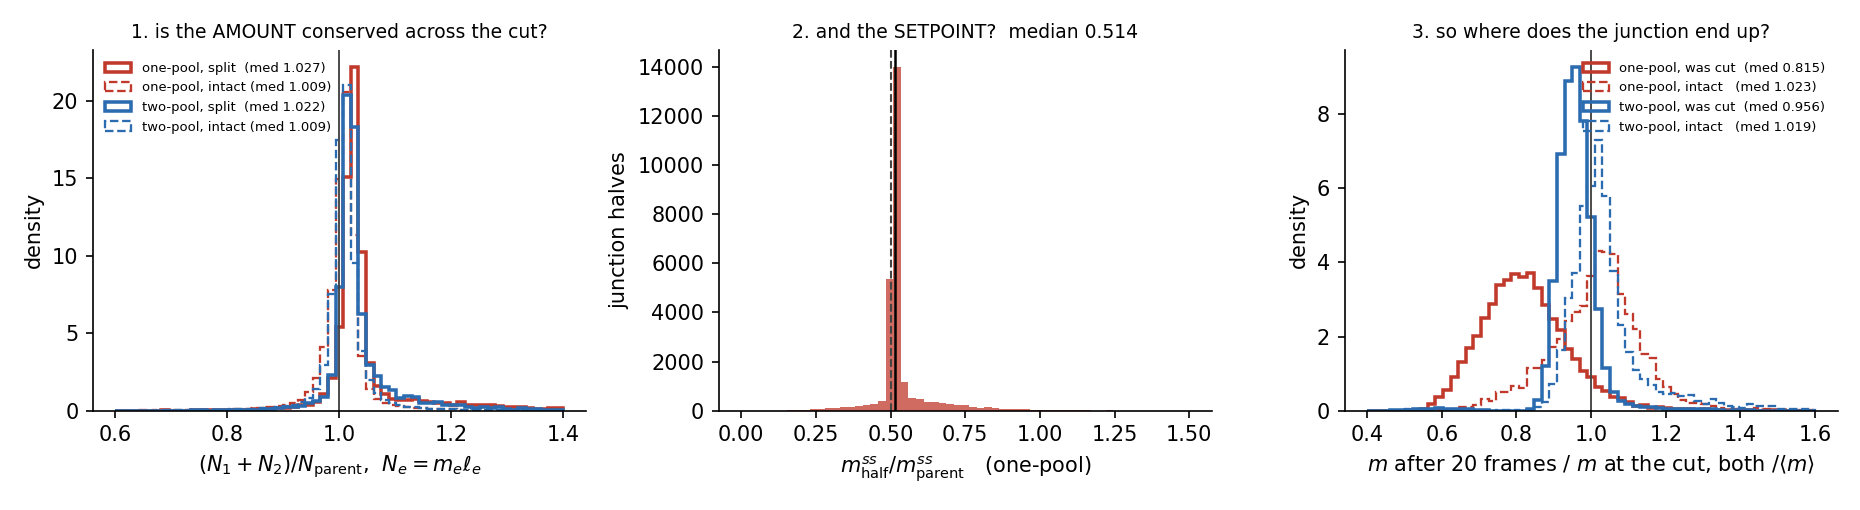
\includegraphics[width=\textwidth]{fig_junction_conservation.png}
\caption{Left: the amount across a cut, both models, against the intact control --- the offset from
$1$ is the $2\%$ by which the two halves are longer than the parent they replace, not a leak. Middle:
the one-pool setpoint of a half over its parent's, which is $1/2$ because the setpoint is proportional
to a length that was just halved. Right: where the junction actually ends up twenty frames later. The
one-pool cut junctions sit $20\%$ below their intact neighbours for no physical reason; the two-pool
ones sit $6\%$ below.}
\end{figure}

\begin{figure}[h]\centering
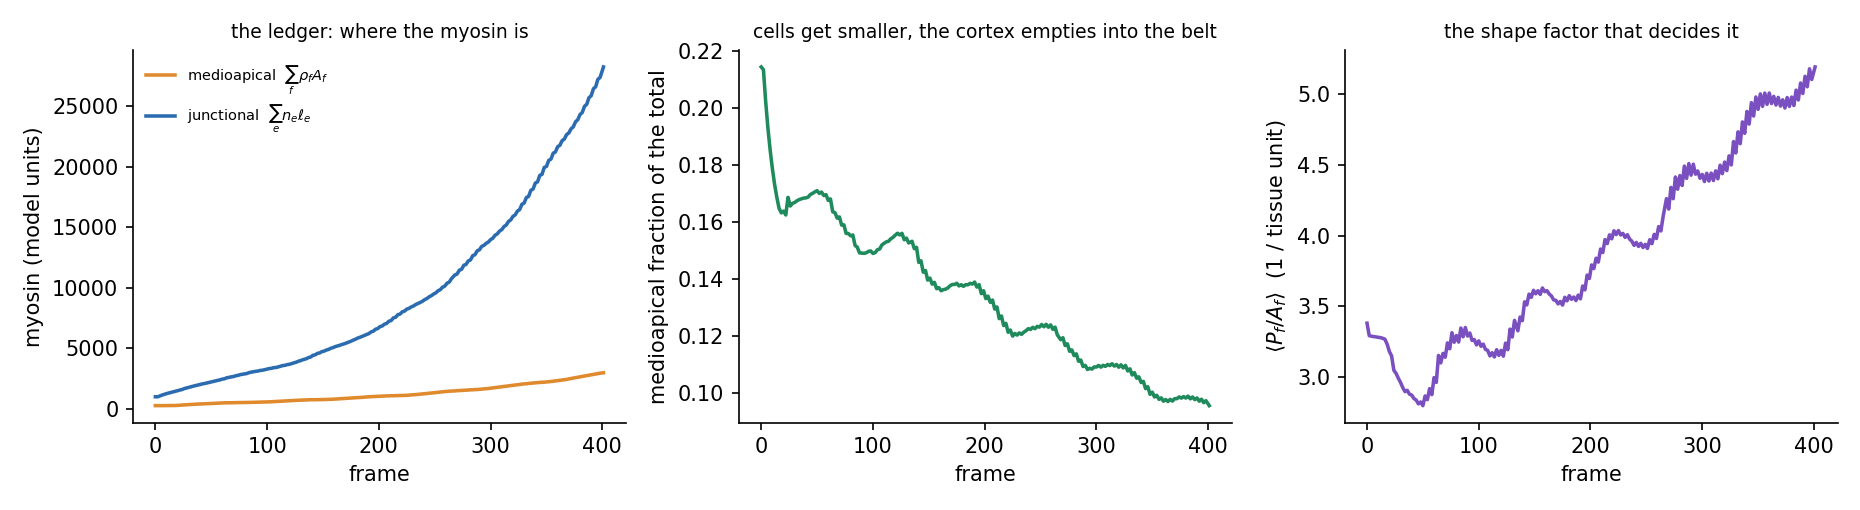
\includegraphics[width=\textwidth]{fig_junction_pools.png}
\caption{The two-pool ledger. Left: both pools grow with the tissue. Middle: the medioapical share
falls from $0.214$ to $0.096$. Right: why --- the mean shape factor $\langle P_f/A_f\rangle$ rises
from $3.38$ to $5.19$ as cells get smaller, and the steady state of Eq.~\eqref{eq:med} depends on it.
Nothing in the specification says myosin should move from the cortex to the belt; the geometry does.}
\end{figure}

\textbf{The residual $6\%$ is not a leftover artifact.} Writing $N_e=n_e\ell_e$ in Eq.~\eqref{eq:jun}
gives $\dot n_e = k_{\text{ex}}\rho - n_e/\tau_{\text{jun}} - n_e\,\mathrm{d}\ln\ell_e/\mathrm{d}t$:
a junction whose length is \emph{changing} dilutes or concentrates its own belt. Freshly cut halves
relax and lengthen, so they dilute. That term is advection of a conserved species along a moving
cable, which is physics; the $20\%$ it replaces was arithmetic.

\section*{6.\; The newborn junction, which the movie found before the measurement did}

Watching \code{01b}'s movie raises a question the tables above do not answer: junctions light up at a
division. They do --- and both the brightness and its location are wrong.

\textbf{What is bright is the wrong junction.} Measured as $m/\langle m\rangle$ at the snapshot after a
division: survivors $1.021$, the two \emph{halves} of a cut contact $1.066$, and the
daughter--daughter interface $0.628$. The halves are enriched because the junction a division cuts is
not a random one --- it sits on a cell that has doubled its volume, so it is $1.24\times$ longer than
average and its cell, being large, has a low $P_f/A_f$, holds more cortical myosin and feeds its belts
harder. That is Eq.~\eqref{eq:med} working correctly. But the place a real dividing cell puts almost
all of its myosin is the \emph{cytokinetic ring}, which constricts exactly at the nascent interface;
in epithelia the new adherens junction is built out of it, with the neighbouring cell contributing
(Herszterg et al., Dev.\ Cell 24:256, 2013; Founounou et al., Dev.\ Cell 24:242, 2013). The model's
division sites were bright in the wrong place and dark in the right one.

\textbf{Why the newborn was dark: a units accident.} \code{myo\_new} was an \emph{absolute} line
density in a model whose mean line density runs $1.07\to1.97\to1.48$ over $401$ frames, so what a new
junction started with was decided by the frame index. The run-median hides this; binning by time does
not --- the newborn's $m/\langle m\rangle$ climbs $0.479\to0.670$ across the run, a $40\%$ drift with
no mechanism behind it.

\textbf{The repair, and what owns it.} A newborn's starting density is a \emph{mechanism}, so it
belongs to an operator rather than to a fallback constant: \code{cytokinetic\_ring} (Structural, on
\code{junction}) seeds every interface with both endpoints new --- exactly the case
\code{\_lookup}'s inheritance already excludes --- at
%
\begin{equation}
n_e = \texttt{ring}\times n^{\ast}, \qquad
n^{\ast}=\tau_{\text{jun}}\,k_{\text{ex}}\,(\rho_f+\rho_g),
\label{eq:ring}
\end{equation}
%
and \emph{debits} the medioapical pools of the two daughters, so the ring moves myosin instead of
creating it and the ledger of \S5 still closes. $n^{\ast}$ is two-sided because a junction is fed by
both cells it separates; the one-sided version was wrong by exactly the factor of two it was meant to
repair, and moved the newborn from $0.628$ to $0.625$, i.e.\ nothing.

\begin{center}\small
\begin{tabular}{@{}lcccl@{}}\toprule
$m/\langle m\rangle$ & absolute & \texttt{ring}$\,=\!1$ & \texttt{ring}$\,=\!3$ & \\\midrule
survivor & $1.021$ & $0.999$ & $0.937$ & the normalisation is shared: bright newborns dim the rest\\
split half & $1.066$ & $1.057$ & $0.964$ & \\
\textbf{newborn interface} & $\mathbf{0.628}$ & $\mathbf{0.920}$ & $\mathbf{2.483}$ & \\
drift across the run & $0.33$ & $0.12$ & $0.09$ & (max$-$min)/median of the newborn, binned by frame\\
T1 per cell per frame & $0.00373$ & $0.00313$ & $0.00388$ & \\
\bottomrule
\end{tabular}
\end{center}

\begin{figure}[h]\centering
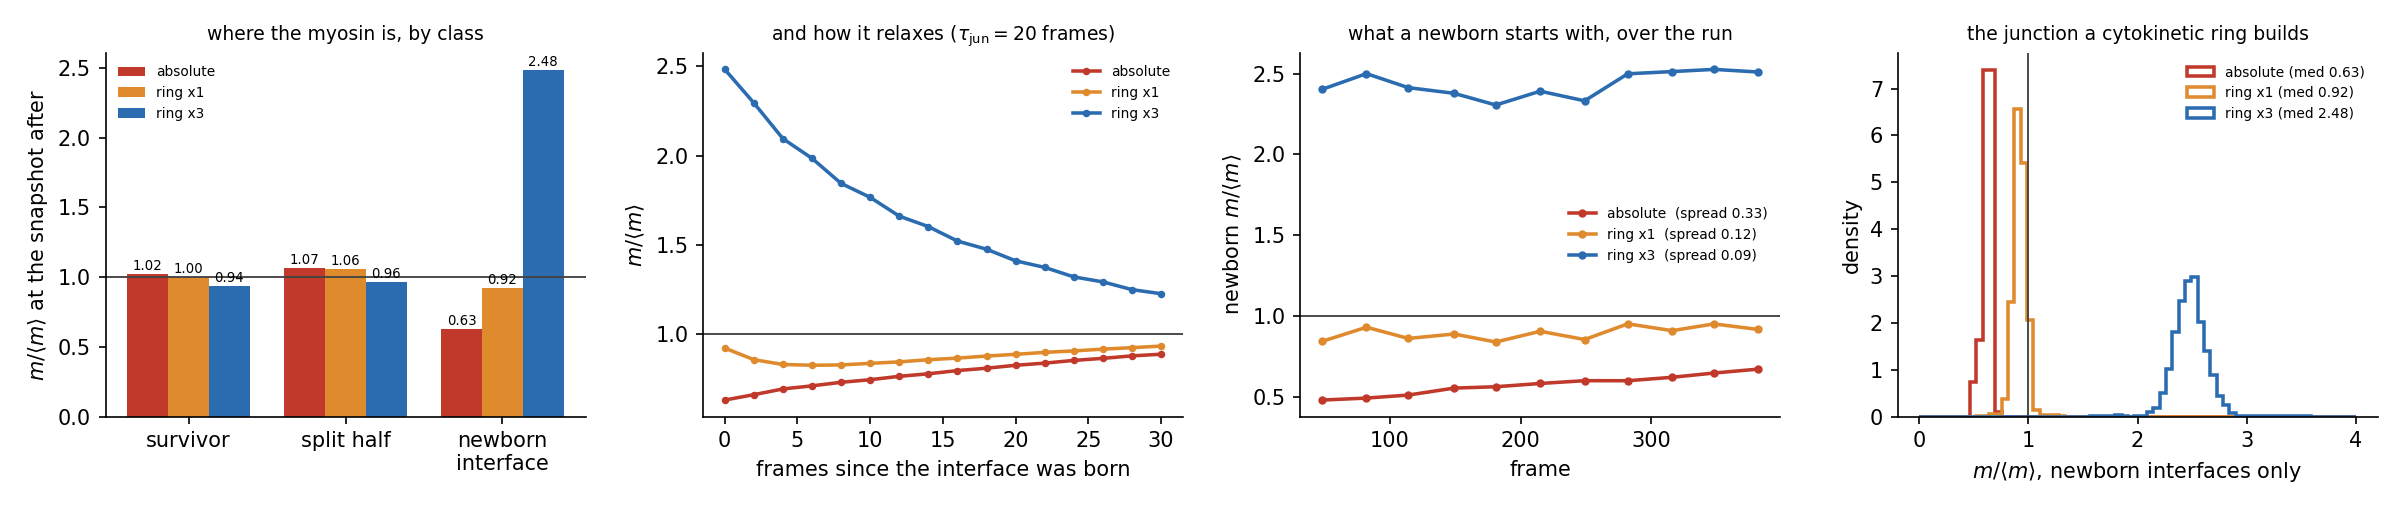
\includegraphics[width=\textwidth]{fig_junction_newborn.png}
\caption{Left: myosin by junction class. Middle-left: the deposit relaxing --- \texttt{ring}$=3$ falls
$2.48\to1.22$ over $30$ frames toward the \texttt{ring}$=1$ level, an $e$-folding of $\sim\!19$ frames
against a $\tau_{\text{jun}}$ of $20$ that nobody fitted: the ring needs no timescale of its own
because the belt already has one. Middle-right: the test of the units repair --- what a newborn starts
with, binned by frame. The absolute rule drifts $0.479\to0.670$; both ring runs are flat. Right: the
distributions.}
\end{figure}

\textbf{Two residuals, both stated rather than tuned away.} At \texttt{ring}$=1$ a newborn sits at
$0.92$ and not $1.00$, because mature junctions are not \emph{at} $n^{\ast}$: the tissue's mean
junction length falls from $0.75$ to $0.46$ as cells divide, and the $-n\,\mathrm{d}\ln\ell/\mathrm{d}t$
term concentrates a shortening belt above its own steady state. The model has no stationary state, and
$8\%$ is what that costs. And without \code{cytokinetic\_ring} in the schedule the seeding falls back
to \code{junction\_myosin}'s scalar, which \code{junction\_myosin\_sync} --- model-agnostic by design
--- renders for the one frame before the belt operator sees it; measured, that put the newborn at
$0.46$ in one part of the run and $0.94$ in another. It is why the control here is \texttt{ring}$=1$
and not ``no ring''.

\section*{7.\; What this does and does not license}

It licenses the reading of $m_e$ as a density and therefore the inheritance rules that were already
written; it licenses the two-pool structure as the smallest thing that makes the junctional setpoint
survive re-meshing, at the cost of one new operator and four rate constants; and it licenses the
claim that the model's own bookkeeping, not its biology, was responsible for a fifth of the myosin on
every junction a division touched.

It does not license the operating point. $k_{\text{on}}$ was set to
$1/\tau_{\text{med}}+k_{\text{ex}}\langle P/A\rangle_0 = 0.219$ so the cortical density \emph{starts}
at its own steady state rather than relaxing to it over the first fifty frames, and
$\tau_{\text{med}}=\tau_{\text{jun}}=20$ frames and $k_{\text{ex}}=0.05$ are chosen numbers, not
measured ones --- and one frame is still not anchored to a time, so ``$20$ frames'' is not yet a claim
about myosin turnover, which is $1$--$2$ minutes. It does not license $\beta_T$: the run reported here
has $\beta_T=0$, pure transport, deliberately, so that a tension bias added later has to beat what
geometry already does. And it does not contain pulsatility, which is the mechanism the medioapical
pool is famous for: Munjal's pulses need advection-mediated positive feedback with dissociation as the
negative arm, which is a third state variable and an advection term. That is the next operator, and
this one is the control it has to beat.

\section*{8.\; What to build next: one specification, three codimensions}

The junction work above is finished, and it makes a specification for the whole spheroid\,--\,basement
membrane\,--\,matrix problem writable. The proposal below is chosen against two constraints at once ---
what the biology requires and what the arithmetic costs --- and both are measured rather than
asserted.

\textbf{Where the time actually goes.} Benchmarked on one A6000, twenty frames each:

\begin{center}\small
\begin{tabular}{@{}lrl@{}}\toprule
body & per frame & note\\\midrule
epithelium, $200\to6900$ cells, $30$ relaxation iterations & $0.22$--$0.52$ s &
$401$ frames in $89$--$210$ s\\
matrix, $9\times10^{4}$ MPM particles, $64^3$ grid, $16$ substeps & $0.92$ s &\\
matrix, $3\times10^{5}$ particles, $64^3$ grid, $16$ substeps & $1.65$ s &\\
matrix, $3\times10^{5}$ particles, $96^3$ grid, $16$ substeps & $1.33$ s & the grid is nearly free\\
\bottomrule
\end{tabular}
\end{center}

Three things follow and they decide the design. The cost is \emph{particles $\times$ substeps} and
almost nothing else --- tripling the grid at fixed particle count did not cost anything measurable, so
resolution in space is cheap and resolution in time is not. The epithelium is a rounding error against
the matrix. And the whole three-body model at $3\times10^{5}$ stroma particles is about
$\mathbf{11}$ \textbf{minutes} for a $401$-frame run: this is not a problem that needs to be made
affordable, it is one that needs to be kept affordable.

\textbf{The specification.} One pass, one \code{Hierarchy}, each body at the codimension its biology
has:

\begin{center}\footnotesize
\begin{tabular}{@{}llll@{}}\toprule
set & kind & one element is & carries\\\midrule
\code{cell} & node & an epithelial cell & $A,P,V$ + targets, $\rho_f$ (medioapical myosin), age\\
\code{vertex} & node & a corner of the apical mesh & \code{pos}\\
\code{junction} & \textbf{edge} $\subseteq$\code{vertex}$^2$ & a cell--cell contact & $n_e$ (line
density), $\ell_e$\\\midrule
\code{bm} & node on a \emph{surface} mesh & a patch of basement membrane & \code{pos},
$\mathbf{F}$, $\rho$ (areal collagen IV), age\\
\code{bm\_edge} & \textbf{edge} $\subseteq$\code{bm}$^2$ & in-plane sheet elasticity & rest length,
$E(\lambda)$\\
\code{plaque} & \textbf{edge} \code{cell}$\to$\code{bm} & one hemidesmosome & $\ell_0$, load, bound\\
\code{fibril} & \textbf{edge} \code{bm}$\to$\code{mpm\_particle} & one anchoring fibril & rest length,
load\\\midrule
\code{mpm\_particle} & node & a patch of \emph{stroma only} & \code{pos}, $\mathbf{F}$, fibre direction\\
\code{mpm\_grid} & field & the stroma's momentum & mass, momentum\\
\bottomrule
\end{tabular}
\end{center}

with the schedule split at exactly one place:
%
\begin{align*}
\text{frame } (\Delta t=1):\quad
&\op{cell\_geometry\_3d}\to\op{grow\_3d}\to\op{bm\_growth\_gate}\\
&\to\op{medioapical\_myosin}\to\op{junction\_myosin}\to\op{shape\_energy\_3d}\\
&\to\op{reconnect\_t1\_3d}\to\op{divide\_3d}\to\op{cytokinetic\_ring}\to\op{junction\_myosin\_sync}\\
&\to\op{bm\_secrete}\to\op{bm\_degrade}\to\op{plaque\_seed}\to\op{plaque\_rupture}\\[3pt]
\text{substep } (\Delta t_{\text{sub}}=\Delta t/16):\quad
&\op{bm\_stiffness}\to\op{bm\_elastic}\to\op{plaque\_pull}\to\op{fibril\_pull}\\
&\to\op{mpm\_strain}\to\op{mpm\_scatter}\to\op{mpm\_grid\_update}\to\op{mpm\_gather}
\end{align*}

\textbf{Four rules, and each buys something specific.}

\emph{1. The basement membrane never enters the grid.} It is $\sim\!100$ nm thick against a
$\sim\!100\,\mu$m spheroid. Resolving that as MPM material needs $\Delta x\lesssim50$ nm over a
$200\,\mu$m domain, i.e.\ $4000^3$ cells --- not slow, impossible. As a surface mesh with its own
in-plane elasticity it costs what the epithelium costs, and $\Delta x$ is then set by the stroma
alone. \S3 of the companion note licenses this: particle-to-surface contact (ICFEMP) exchanges force
conservatively at a resolution where grid-node coupling cannot, measured to $1.4\times10^{-7}$
relative momentum residual.

\emph{2. The epithelium stays out of the substep block.} It is overdamped and has no mass, so it does
not need the matrix's CFL step; putting its $30$-iteration relaxation inside the loop would multiply
its cost by $16$ and change nothing. This is what the \code{substep\_dt} block is for, and it is the
whole reason a stiff continuum and a quasi-static tissue can share one specification.

\emph{3. Keep the sheet massless too, and its stiffness costs drag rather than substeps.} The
literature wants $E_{\text{bm}}/E_{\text{ecm}}\in[10,100]$, and a stiff \emph{inertial} sheet inside
the substep block would set $n_{\text{sub}}$ by itself. Overdamped, the bound is
$\Delta t\,(z k_b+\kappa)/\gamma<2$ --- a rate, not a wave speed --- so the ratio is paid for with
$\gamma$ and the substep count stays the stroma's.

\emph{4. Spend particles on the shell that carries stress, not on the box.} The far field is
quiescent; $3\times10^{5}$ particles in a shell around the spheroid resolve the gradient that the
growth gate reads, and the grid can be refined for free (rule above) if the sheet's imprint needs it.

\textbf{What it deletes, which is the other half of the leverage.} The \code{surface} Level and the
two-pass structure go: once \op{plaque\_pull} returns its reaction, the epithelium is pushed back and
there is no recorded boundary to consult. \op{cell\_to\_ecm} and \op{cell\_exclude\_3d} go with them
--- while the sheet is intact the basement membrane \emph{is} the interface, and an epithelium that
also pushes the stroma is counting the same push twice. And MPM fibres stop being asked to act as
ropes, which \S7 of \code{spheroid\_ecm.tex} measured they cannot.

\textbf{One thing this makes newly uncomfortable, and it belongs here rather than in a footnote.}
The specification above forces a frame to have a duration, because \op{bm\_secrete} is a mass balance
with $\tau_{\text{bm}}=4$--$14$ h in it. The run's own growth fixes it: $200\to6900$ cells is $5.1$
doublings, so at a $12$--$24$ h cycle the $401$ frames are $2.5$--$5$ days and one frame is
$9$--$18$ minutes. Collagen IV turnover is then $13$--$93$ frames --- comfortably resolved, which is
the good news. Junctional myosin turnover is $1$--$2$ \emph{minutes}, i.e.\ a tenth of a frame: at this
resolution the belt is adiabatic, $n_e$ should be its steady state every frame, and
$\tau_{\text{jun}}=20$ frames is not myosin turnover by two orders of magnitude. What a $20$-frame
memory on a junction can legitimately be is \emph{maturation} --- E-cadherin accumulation and the
assembly of a new contact, which run over tens of minutes to hours --- so the parameter should be
renamed, re-sourced, and separated from the turnover it is currently pretending to be. That is the
first thing to fix in the model this note just built, and the specification above is what makes the
question askable at all.

\end{document}
